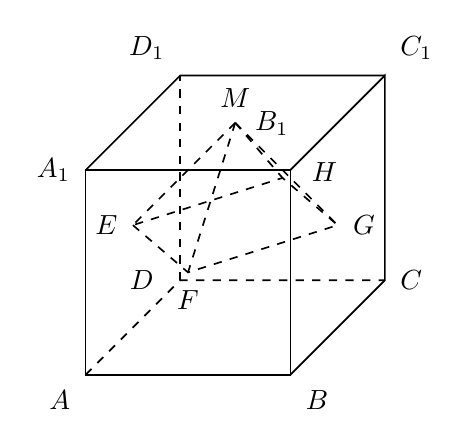
\begin{tikzpicture}[x=1cm,y=1cm,line width=.6pt]
% Cube + inner pyramid M-EFGH, face centers
\coordinate (A) at (0,0);
\coordinate (B) at (2.6,0);
\coordinate (B1) at (2.6,2.6);
\coordinate (A1) at (0,2.6);
\coordinate (D) at (1.2,1.2);
\coordinate (C) at (3.8,1.2);
\coordinate (D1) at (1.2,3.8);
\coordinate (C1) at (3.8,3.8);
% face centers: M top, E left, F front, G right, H back
\coordinate (M) at (1.9,3.2);
\coordinate (E) at (0.6000000000,1.9000000000);
\coordinate (F) at (1.3000000000,1.3000000000);
\coordinate (G) at (3.2000000000,1.9000000000);
\coordinate (H) at (2.5000000000,2.5000000000);
% solid cube
\draw (A) -- (B) -- (B1) -- (A1) -- cycle;
\draw (B) -- (C) -- (C1) -- (B1);
\draw (A1) -- (D1) -- (C1);

% inner pyramid all dashed
\draw[dashed] (E) -- (F) -- (G) -- (H) -- cycle;
\draw[dashed] (M) -- (E);
\draw[dashed] (M) -- (F);
\draw[dashed] (M) -- (G);
\draw[dashed] (M) -- (H);
% hidden cube
\draw[dashed] (A) -- (D) -- (C);
\draw[dashed] (D) -- (D1);

% labels
\node[below left=2pt] at (A) {$A$};
\node[below right=2pt] at (B) {$B$};
\node[right=2pt] at (C) {$C$};
\node[left=6pt] at (D) {$D$};
\node[left=2pt] at (A1) {$A_{1}$};
\node[above left=2pt,xshift=5pt,yshift=7pt] at (B1) {$B_{1}$};
\node[above right=2pt] at (C1) {$C_{1}$};
\node[above left=2pt] at (D1) {$D_{1}$};
\node[above=2pt] at (M) {$M$};
\node[left=2pt] at (E) {$E$};
\node[below=3pt] at (F) {$F$};
\node[right=2pt] at (G) {$G$};
\node[above right=2pt,xshift=5pt,yshift=-7pt] at (H) {$H$};
\end{tikzpicture}
